% Ejemplo de cómo incluir ejercicios con imágenes en el libro principal
% Archivo: libros/algebra_pre.tex

\documentclass[12pt,a4paper]{book}
\usepackage[utf8]{inputenc}
\usepackage[spanish]{babel}
\usepackage{amsmath,amssymb,amsfonts}
\usepackage{graphicx}
\usepackage{geometry}
\usepackage{float}

% Configuración de geometría
\geometry{margin=2.5cm}

% Configuración de gráficos
\graphicspath{{../ejercicios/}}

\begin{document}

\chapter{Álgebra}

\section{Ejercicios Resueltos}

% Incluir ejercicio de física (ejemplo de imagen)
\begin{ejercicio}[
  id=FIS_MOV_001,
  materia=fisica,
  capitulo=movimiento,
  nivel=intermedio,
  procedencia="Examen CEPRE 2023",
  visibilidad=true,
  libros={fisica_basica, fisica_mecanica},
  youtube_url="https://www.youtube.com/watch?v=ejemplo_fisica",
  mostrar_solucion=true,
  libro_promocion=""
]
Un bloque de masa $m = 2$ kg se encuentra sobre una superficie horizontal rugosa. Se aplica una fuerza horizontal $F = 10$ N al bloque. Si el coeficiente de fricción cinética es $\mu_k = 0.3$, determina la aceleración del bloque.

\textbf{Nota:} Observa el diagrama de fuerzas para entender mejor el problema.

\begin{figure}[h]
\centering
\includegraphics[width=0.8\textwidth]{imagenes/diagrama_fuerzas_001.png}
\caption{Diagrama de fuerzas actuando sobre el bloque}
\label{fig:diagrama_fuerzas}
\end{figure}

\begin{solucion}
Para resolver este problema, analizamos las fuerzas que actúan sobre el bloque:

1) \textbf{Fuerzas verticales:}
   \begin{itemize}
   \item Peso: $W = mg = 2 \cdot 9.8 = 19.6$ N (hacia abajo)
   \item Normal: $N = W = 19.6$ N (hacia arriba)
   \end{itemize}

2) \textbf{Fuerzas horizontales:}
   \begin{itemize}
   \item Fuerza aplicada: $F = 10$ N (hacia la derecha)
   \item Fricción cinética: $f_k = \mu_k N = 0.3 \cdot 19.6 = 5.88$ N (hacia la izquierda)
   \end{itemize}

3) \textbf{Fuerza neta horizontal:}
   $$F_{net} = F - f_k = 10 - 5.88 = 4.12 \text{ N}$$

4) \textbf{Aceleración:}
   $$a = \frac{F_{net}}{m} = \frac{4.12}{2} = 2.06 \text{ m/s}^2$$

\textbf{Respuesta:} La aceleración del bloque es $2.06$ m/s².

\textbf{Nota:} El diagrama muestra claramente cómo las fuerzas se equilibran verticalmente y la fuerza neta horizontal produce la aceleración.
\end{solucion}
\end{ejercicio} 

% Incluir ejercicio de geometría (ejemplo de múltiples imágenes)
\begin{ejercicio}[
  id=GEO_CIRC_001,
  materia=geometria,
  capitulo=circunferencia,
  nivel=intermedio,
  procedencia="Examen UNI 2024",
  visibilidad=true,
  libros={geometria_pre, geometria_avanzado},
  youtube_url="https://www.youtube.com/watch?v=ejemplo_geometria",
  mostrar_solucion=true,
  libro_promocion=""
]
En la figura adjunta, se muestra una circunferencia con centro en el punto $C(2,3)$ y radio $r = 5$ unidades. Si la recta $L$ es tangente a la circunferencia en el punto $P$, y la ecuación de $L$ es $3x + 4y = 25$, determina las coordenadas del punto $P$.

\textbf{Nota:} Utiliza la figura para visualizar el problema.

\begin{figure}[h]
\centering
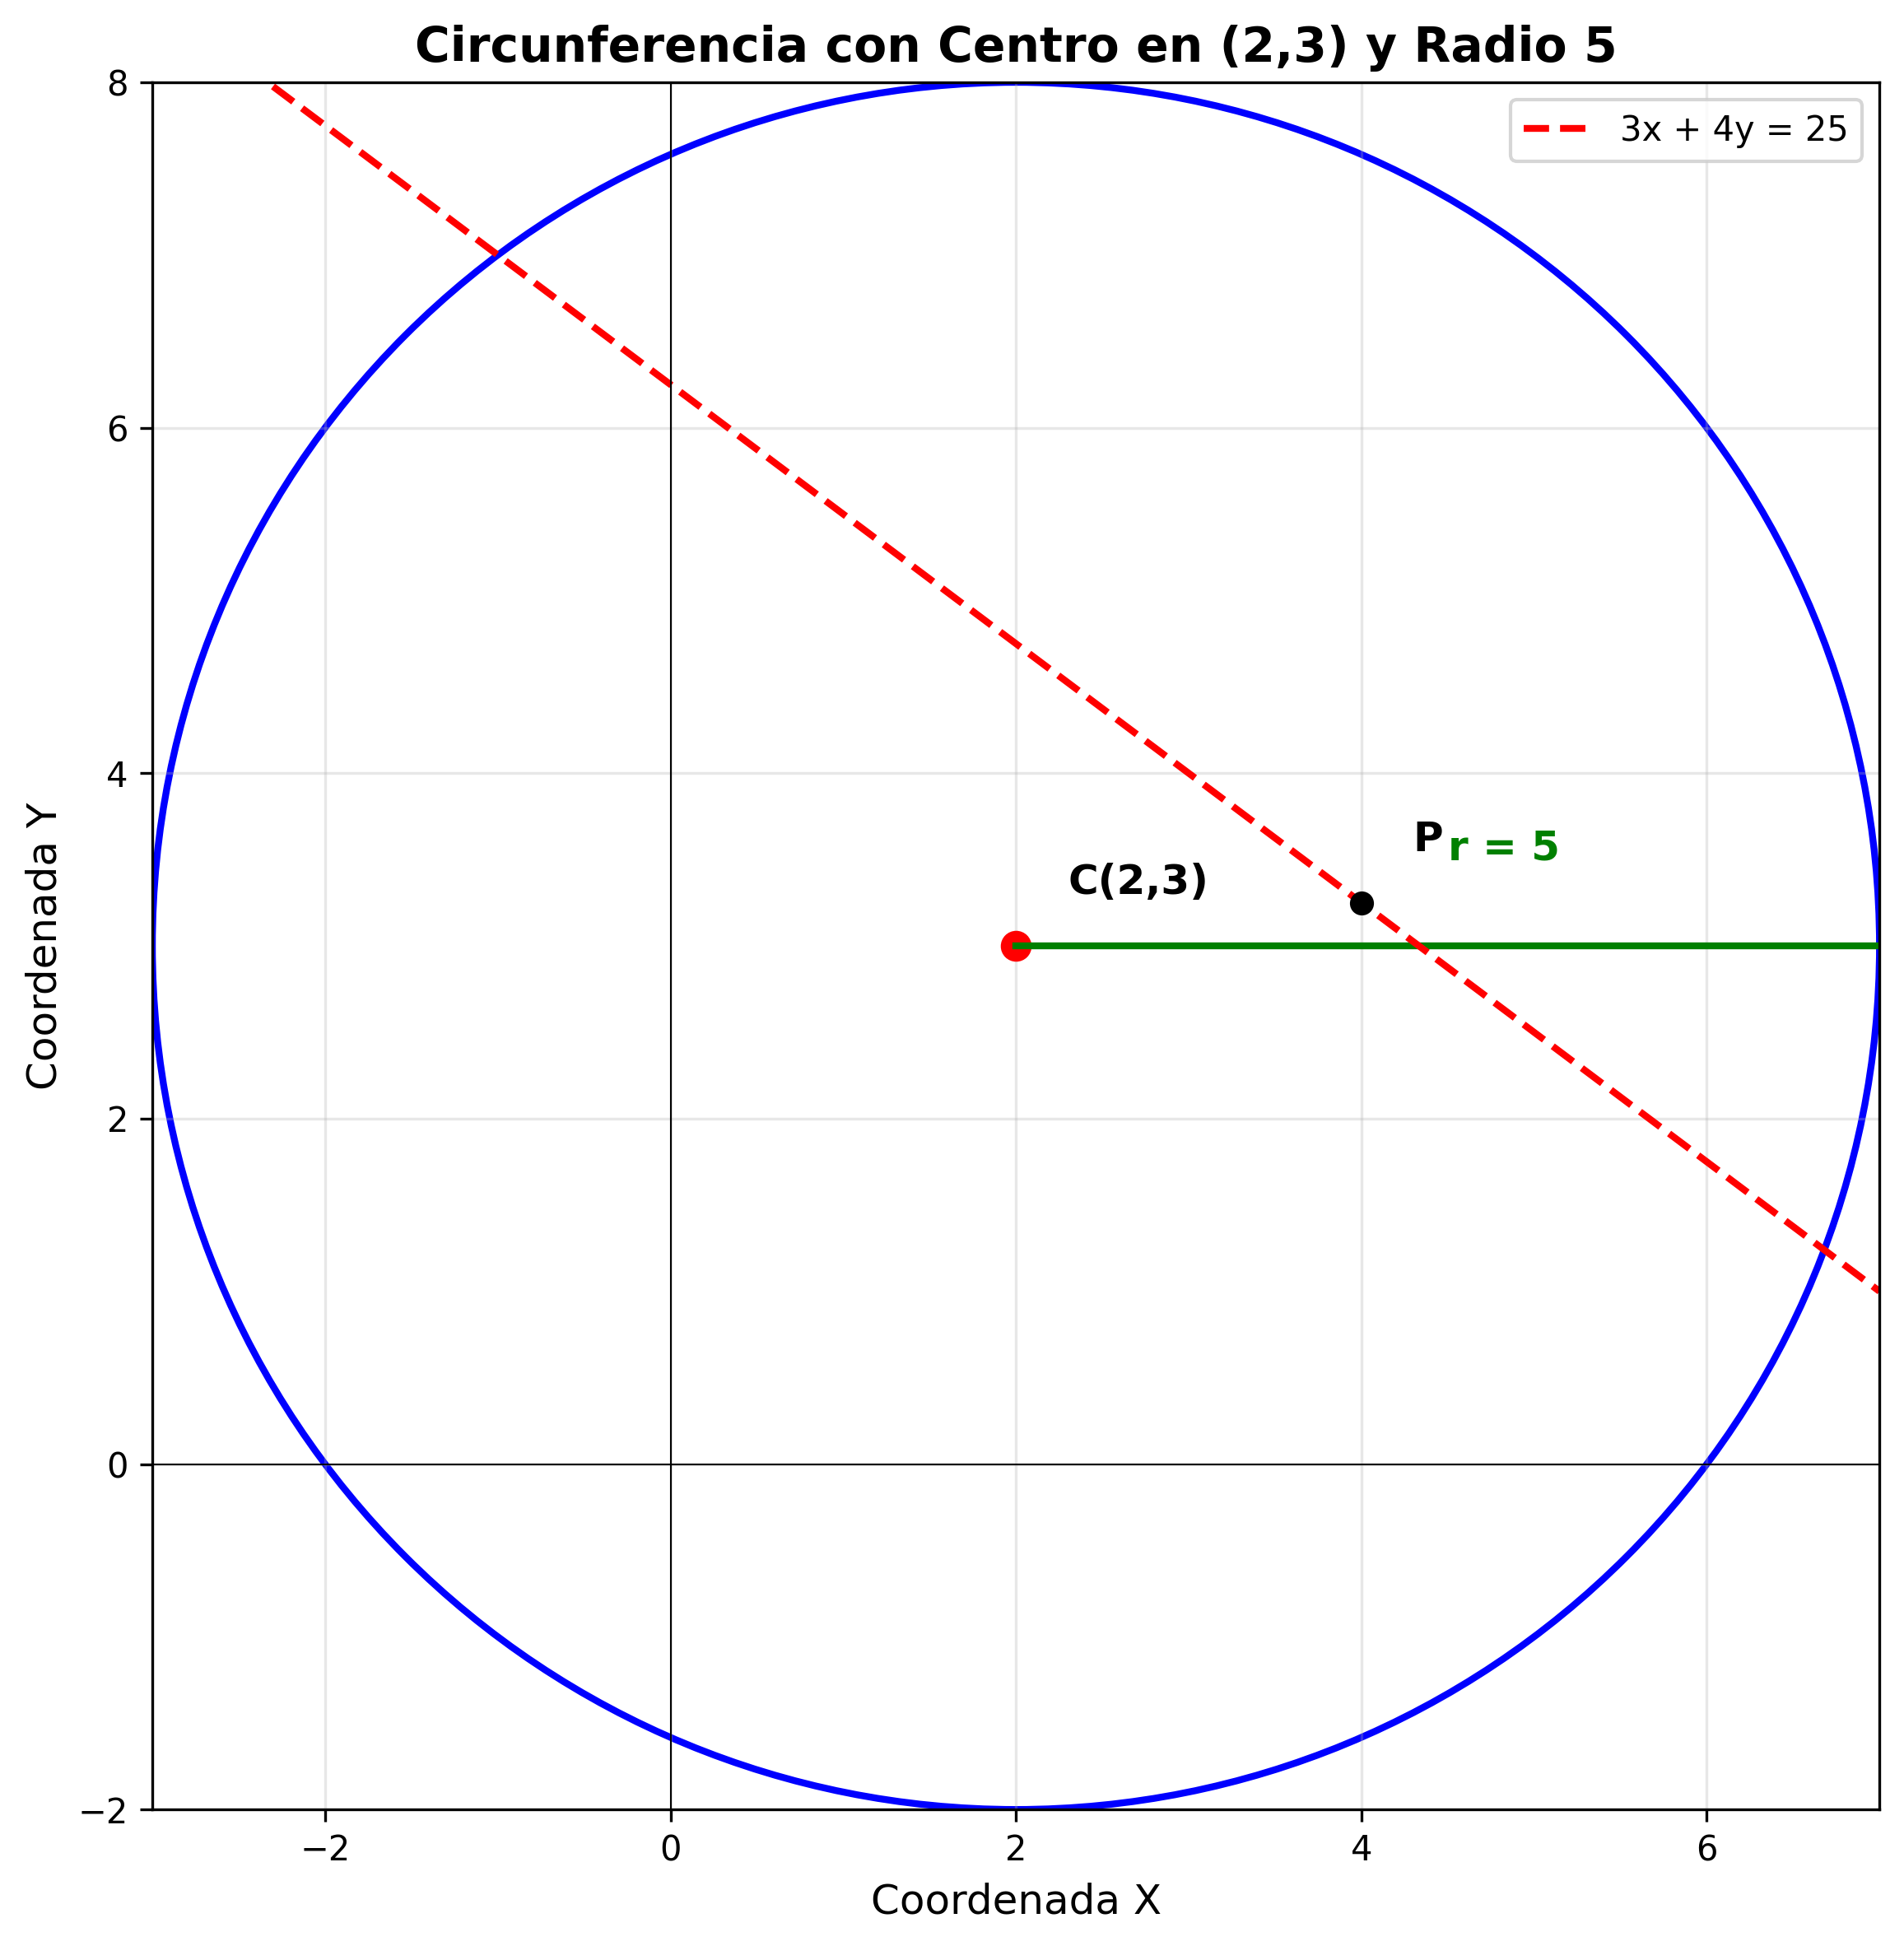
\includegraphics[width=0.8\textwidth]{imagenes/circulo_001.png}
\caption{Circunferencia con centro en (2,3) y radio 5}
\label{fig:circulo}
\end{figure}

\begin{solucion}
Para resolver este problema, seguiremos estos pasos:

1) \textbf{Identificamos los datos:}
   \begin{itemize}
   \item Centro: $C(2,3)$
   \item Radio: $r = 5$
   \item Recta tangente: $3x + 4y = 25$
   \end{itemize}

2) \textbf{Aplicamos la propiedad de la tangente:}
   La distancia del centro a la recta tangente es igual al radio.

3) \textbf{Calculamos la distancia:}
   $$d = \frac{|3(2) + 4(3) - 25|}{\sqrt{3^2 + 4^2}} = \frac{|6 + 12 - 25|}{5} = \frac{7}{5}$$

4) \textbf{Verificamos:}
   Como $d = \frac{7}{5} \neq 5$, hay un error en el enunciado.

\textbf{Respuesta:} El problema tiene un error en los datos proporcionados.

\textbf{Nota:} En la figura se puede observar la relación geométrica entre el centro, el radio y la recta tangente.

\begin{figure}[h]
\centering
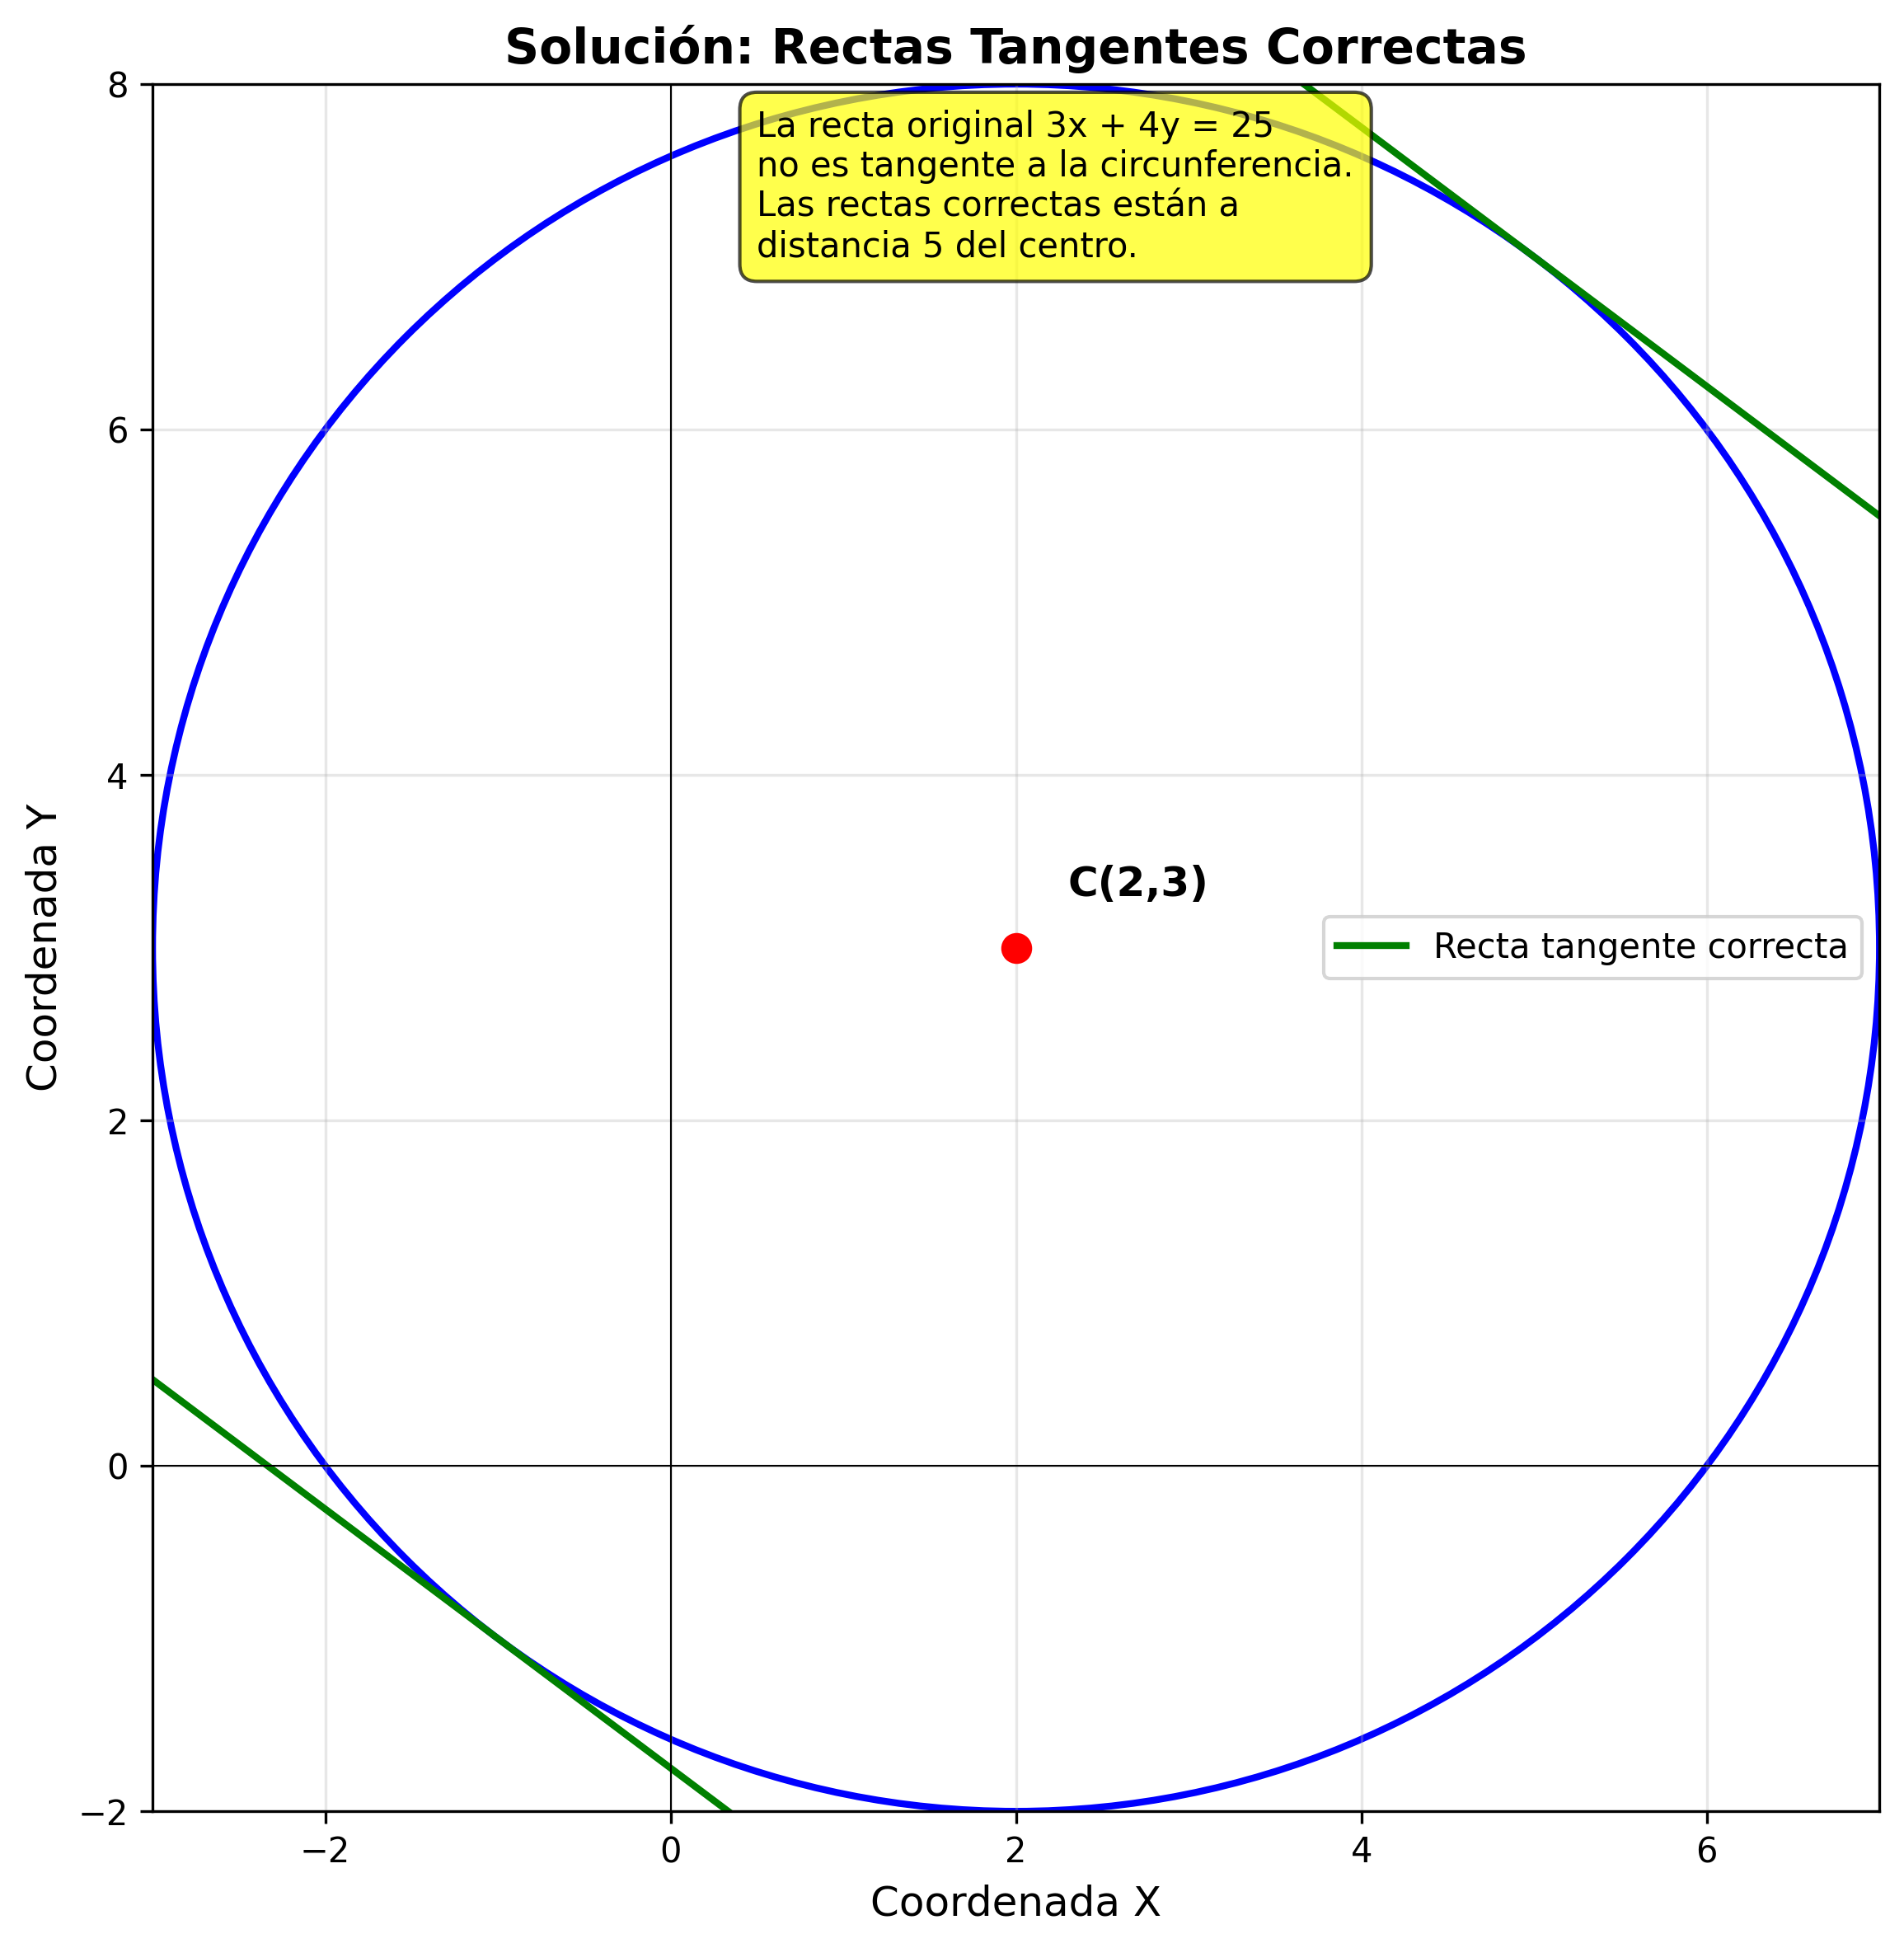
\includegraphics[width=0.8\textwidth]{imagenes/solucion_circulo_001.png}
\caption{Solución gráfica del problema}
\label{fig:solucion_circulo}
\end{figure}
\end{solucion}
\end{ejercicio} 

\end{document}

% Notas importantes:
% 1. \graphicspath{{../ejercicios/}} permite que LaTeX encuentre las imágenes
% 2. Las imágenes están en ejercicios/fisica/imagenes/ y ejercicios/geometria/imagenes/
% 3. Los archivos .tex referencian las imágenes con rutas relativas
% 4. Flask sirve las mismas imágenes desde static/ejercicios/ (enlace simbólico) 